\documentclass[handout,compress]{beamer}

\usetheme[block=fill]{metropolis}

\usepackage{graphicx} % Allows including images
\usepackage{amsmath,amsfonts,amsthm,amssymb}
\usepackage{color}
\usepackage{xcolor,cancel}
%\setitemize{label=\usebeamerfont*{itemize item}%
%	\usebeamercolor[fg]{itemize item}
%	\usebeamertemplate{itemize item}}
\definecolor{mDarkBrown}{HTML}{604c38}
\definecolor{mDarkTeal}{HTML}{23373b}
\definecolor{mLightBrown}{HTML}{EB811B}
\definecolor{mMediumBrown}{HTML}{C87A2F}
\definecolor{mygreen}{HTML}{98C2B9}
\definecolor{myyellow}{HTML}{DFD79C}
\definecolor{myblue}{HTML}{8CA7CC}
\definecolor{kern}{HTML}{8CC2B7}

\usepackage{float}
\usepackage{framed}
\usepackage{epsfig}
\usepackage{graphicx}
\usepackage{subcaption}
\usepackage{ulem}
\usepackage{hhline}
\usepackage{multirow}
\usepackage{comment}   
\usepackage{bbm}
\usepackage{tikz}   
\def\Put(#1,#2)#3{\leavevmode\makebox(0,0){\put(#1,#2){#3}}}
\newcommand*\mystrut[1]{\vrule width0pt height0pt depth#1\relax}
\newcommand{\eqdef}{\mathbin{\stackrel{\rm def}{=}}}


\newcommand{\bs}[1]{\boldsymbol{#1}}
\newcommand{\bv}[1]{\mathbf{#1}}
\newcommand{\R}{\mathbb{R}}
\newcommand{\E}{\mathbb{E}}

\DeclareMathOperator*{\argmin}{arg\,min}
\DeclareMathOperator*{\argmax}{arg\,max}
\DeclareMathOperator{\nnz}{nnz}
\DeclareMathOperator{\Var}{Var}
\DeclareMathOperator{\sinc}{sinc}
\DeclareMathOperator{\mv}{mv}
\DeclareMathOperator{\sgn}{sgn}
\DeclareMathOperator{\step}{step}
\DeclareMathOperator{\gap}{gap}
\DeclareMathOperator{\poly}{poly}
\DeclareMathOperator{\tr}{tr}
\DeclareMathOperator{\orth}{orth}
\newcommand{\norm}[1]{\|#1\|}
\captionsetup[subfigure]{labelformat=empty}
\captionsetup[figure]{labelformat=empty}
\DeclareMathOperator*{\lmin}{\lambda_{min}}
\DeclareMathOperator*{\lmax}{\lambda_{max}}

\newcommand{\specialcell}[2][c]{%
  \begin{tabular}[#1]{@{}c@{}}#2\end{tabular}}
\newcommand{\specialcellleft}[2][c]{%
\begin{tabular}[#1]{@{}l@{}}#2\end{tabular}
}

\usepackage{tabstackengine}
\stackMath


%----------------------------------------------------------------------------------------
%	TITLE PAGE
%----------------------------------------------------------------------------------------

\title{CS-UY 4563: Lecture 2 \\ Simple Linear Regression}
\author{NYU Tandon School of Engineering, Prof. Christopher Musco}
\date{}

\begin{document}

\begin{frame}
	\titlepage 
\end{frame}

\metroset{titleformat=smallcaps}

\begin{comment}
\end{comment}

\begin{frame}
	\frametitle{course admin}
	\begin{itemize}
		\item Please enroll for Piazza. Only about $60\%$ of class has. 
		\item First lab assignment: \texttt{lab\_housing\_partial.ipynb} 
		\begin{itemize}
			\item Due \textbf{next Tuesday, 2/4 at 11:59pm}.
			\item Go through the simple regression demonstration \texttt{demo\_auto\_mpg.ipynb}.
			\item Turn in entire Jupyter Notebook via NYU Classes. 
			\item At top of notebook list any collaborators you worked with (as many as you like).
			\item There will be a corresponding written homework released shortly.
		\end{itemize}
	\end{itemize}
	\end{frame}

\begin{frame}
	\frametitle{basic goal}
	\textbf{Goal:} Develop algorithms to make decisions or predictions based on data.
	\begin{itemize}
		\item \textbf{Input:} A single piece of data (an image, audio file, patient healthcare record, MRI scan).
		\begin{center}
		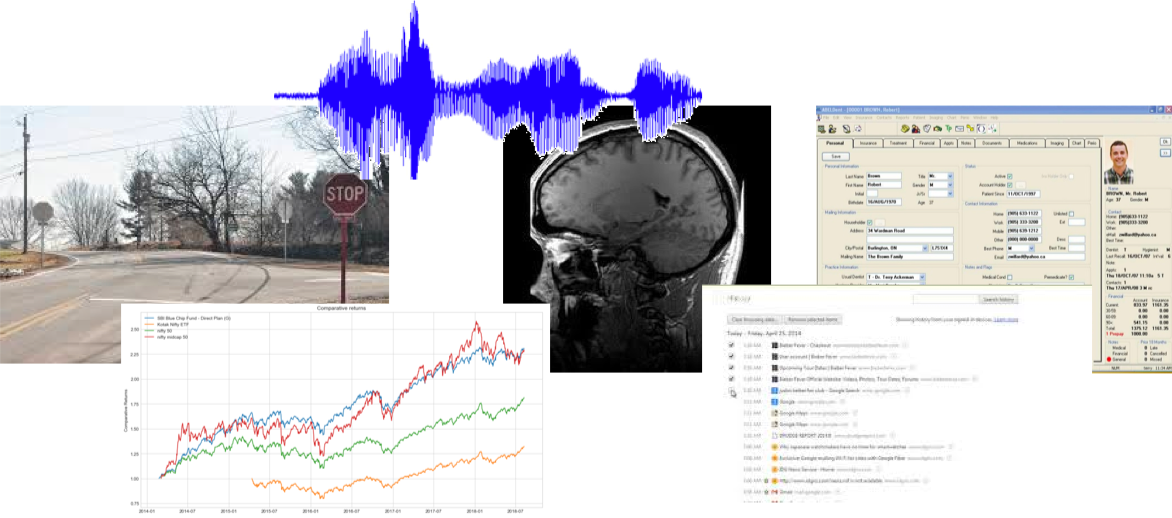
\includegraphics[width=.6\textwidth]{data_examples.png}
		\end{center}
		\item \textbf{Output:} A prediction or decision (this image is a stop sign, this stock will go up $10\%$ next quarter, turn the car right).
	\end{itemize}
\end{frame}


\begin{frame}
	\frametitle{supervised learning}
	\textbf{Step 1:}
	Collect and label many input/output pairs $(\bv{x}_i,y_i)$.
	For our digit images, we have each $\bv{x}_i\in \R^{28\times 28}$ and $y_i \in \{0, 1, \ldots, 9\}$. 
	\begin{center}
		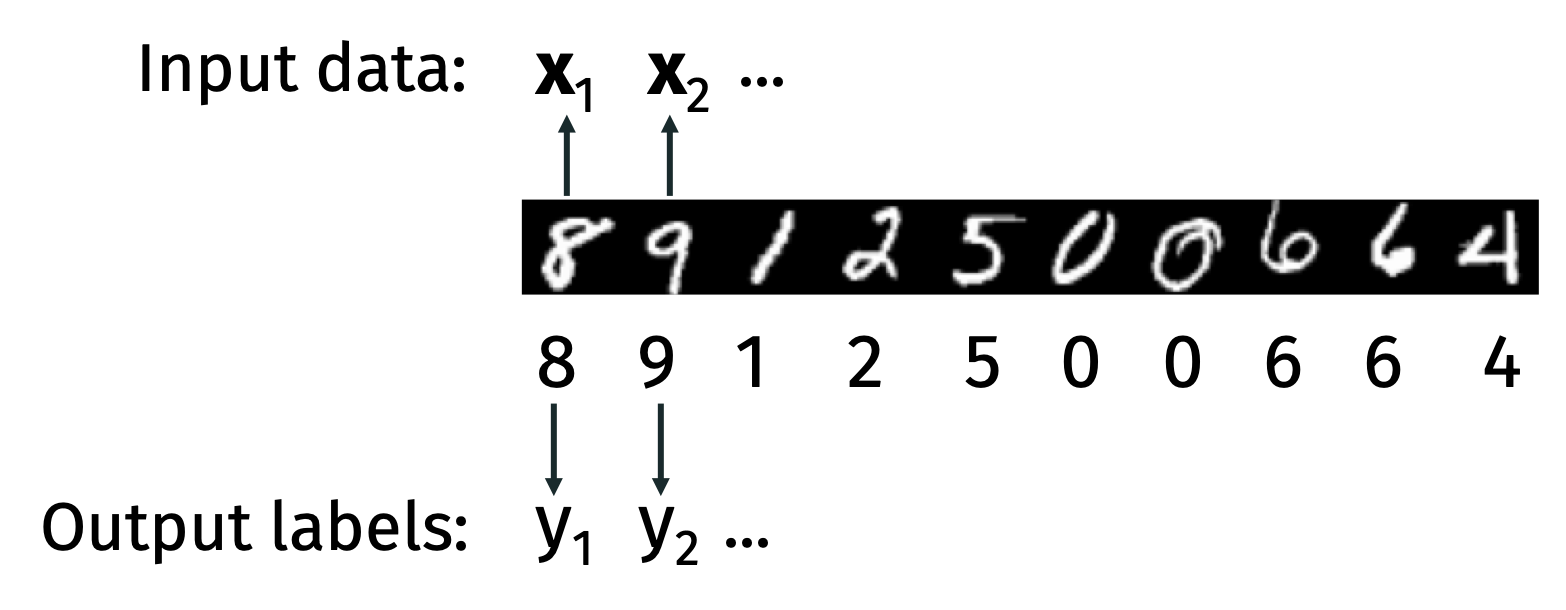
\includegraphics[width=.6\textwidth]{collect_data.png}
	\end{center}
	This is called the \textbf{\alert{training dataset.}}
\end{frame}

\begin{frame}
	\frametitle{supervised}
	\textbf{Step 2:} Learn from the examples we have.
	\begin{itemize}
		\item Have the computer \emph{automatically} find some function $f(\bv{x})$ such that $f(\bv{x}_i) = y_i$ \alert{for most $(\bv{x}_i,y_i)$ in our training data set} (by searching over many possible functions).
	\end{itemize}
\end{frame}


\begin{frame}
	\frametitle{machine learning}
	In \textbf{\alert{supervised learning}} every input $\bv{x}_i$ in our training dataset comes with a desired output $y_i$ (typically generated by a human, or some other process).
	
	Types of {supervised earning:}
	\begin{itemize}
		\item \textbf{Classification} -- predict a \emph{discrete} class label.
		\item \textbf{Regression} -- predict a \emph{continuous} value.
		\begin{itemize}
			\item Dependent variable, response variable, target variable, lots of different names for $y_i$.
		\end{itemize}
	\end{itemize}
\end{frame}

\begin{frame}
	\frametitle{supervised learning}
	Another example of supervised classification: \textbf{Face Detection}.
	\begin{center}
		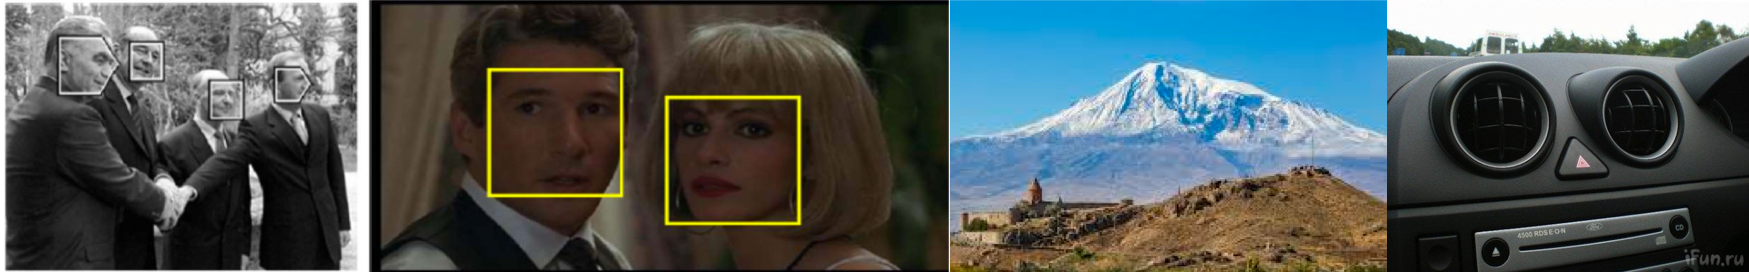
\includegraphics[width=.8\textwidth]{facedetection.png}
	\end{center}
	Each input data example $\bv{x}_i$ is an image. Each output $y_i$ is $1$ if the image contains a face, $0$ otherwise.
	
	\begin{itemize}
		\item Harder than digit recognition, but we now have very reliable methods (used in nearly all digital cameras, phones, etc.)
	\end{itemize}
\end{frame}

\begin{frame}
	\frametitle{supervised learning}
	Other examples of supervised classification:
	\begin{itemize}
		\item \emph{Object detection} (Input: image, Output: dog or cat)
		\item \emph{Spam detection} (Input: email text, Output: spam or not)
		\item \emph{Medical diagnosis} (Input: patient data, Output: disease condition or not)
		\item \emph{Credit decision making} (Input: financial data, Output: offer loan or not)
	\end{itemize}
	
\end{frame}

\begin{frame}
	\frametitle{supervised learning}
	 Example of supervised regression: \textbf{Stock Price Prediction}.
	\begin{center}
		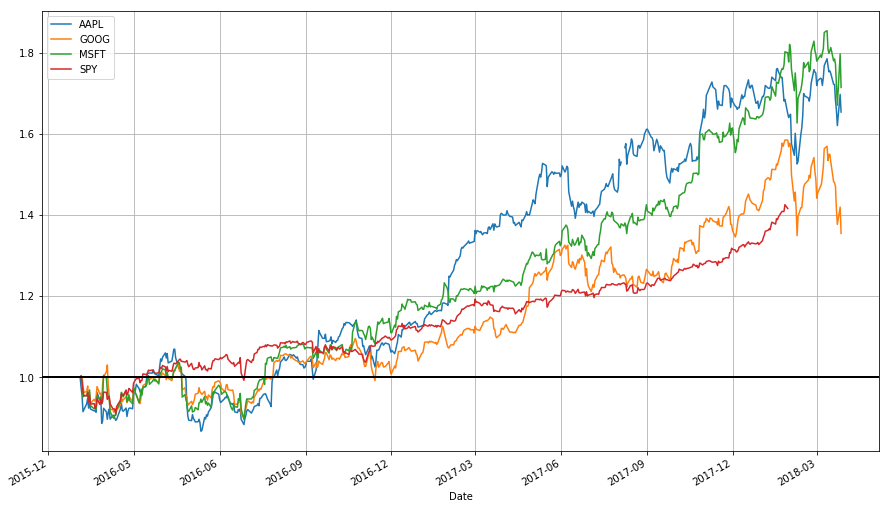
\includegraphics[width=.5\textwidth]{stock_data.png}
	\end{center}
	Each input $\bv{x}$ is a vector of metrics about a company (sales volume, PE ratio, earning reports, historical price data). 
	
	Each output $y_i$ is the \textbf{price of the stock} 3 months in the future. 
\end{frame}

\begin{frame}
	\frametitle{supervised learning}
	Other examples of supervised regression:
	\begin{itemize}
		\item \emph{Home price prediction} (Inputs: square footage, zip code, number of bathrooms, Output: Price)
		\item \emph{Car price prediction} (Inputs: make, model, year, miles driven, Output: Price)
		\item \emph{Weather prediction} (Inputs: weather data at nearby stations, Output: tomorrows temperature )
		\item \emph{Robotics/Control} (Inputs: information about environment and current position at time $t$, Output: estimate of position at time $t+1$)	
	\end{itemize}
\end{frame}

\begin{frame}
	\frametitle{other types of learning}
	Later in the class we will talk about other models: 
	\begin{itemize}
		\item \textbf{Unsupervised learning} (no labels or response variable)
		\begin{itemize}
			\item Clustering
			\item Representation Learning
		\end{itemize}
		\item \textbf{Reinforcement learning}
			\begin{itemize}
				\item Game playing
			\end{itemize}
	\end{itemize}
You might also hear about semi-supervised learning or active learning -- these categories aren't always cut and dry.
\end{frame}

\begin{frame}
	\frametitle{supervised learning}
		In \textbf{supervised learnings} every input $\bv{x}_i$ in our training dataset comes with a desired output $y_i$ (typically generated by a human, or some other process).
		
	Types of {supervised earning:}
	\begin{itemize}
		\item \textbf{Classification} -- predict a \emph{discrete} class label.
		\alert{\item \textbf{Regression} -- predict a \emph{continuous} value.
		\begin{itemize}
			\item Dependent variable, response variable, target variable, lots of different names for $y_i$.
		\end{itemize}}
	\end{itemize}
\end{frame}

\begin{frame}
	\frametitle{predicting mpg}
	\textbf{Motivating example:} Predict the highway miles per gallon (MPG) of a car given quantitative information about its engine. Demo in
	\texttt{\href{https://github.com/cpmusco/introml/tree/master/simple_linear_regression}{demo\_auto\_mpg.ipynb}}.
	\vspace{4em}
	
	
	\textbf{What factors might matter?}
	\vspace{4em}
\end{frame}

\begin{frame}
	\frametitle{predicting mpg}
	Data set available from the UCI Machine Learning Repository: \href{https://archive.ics.uci.edu/}{https://archive.ics.uci.edu/}.
	\begin{center}
		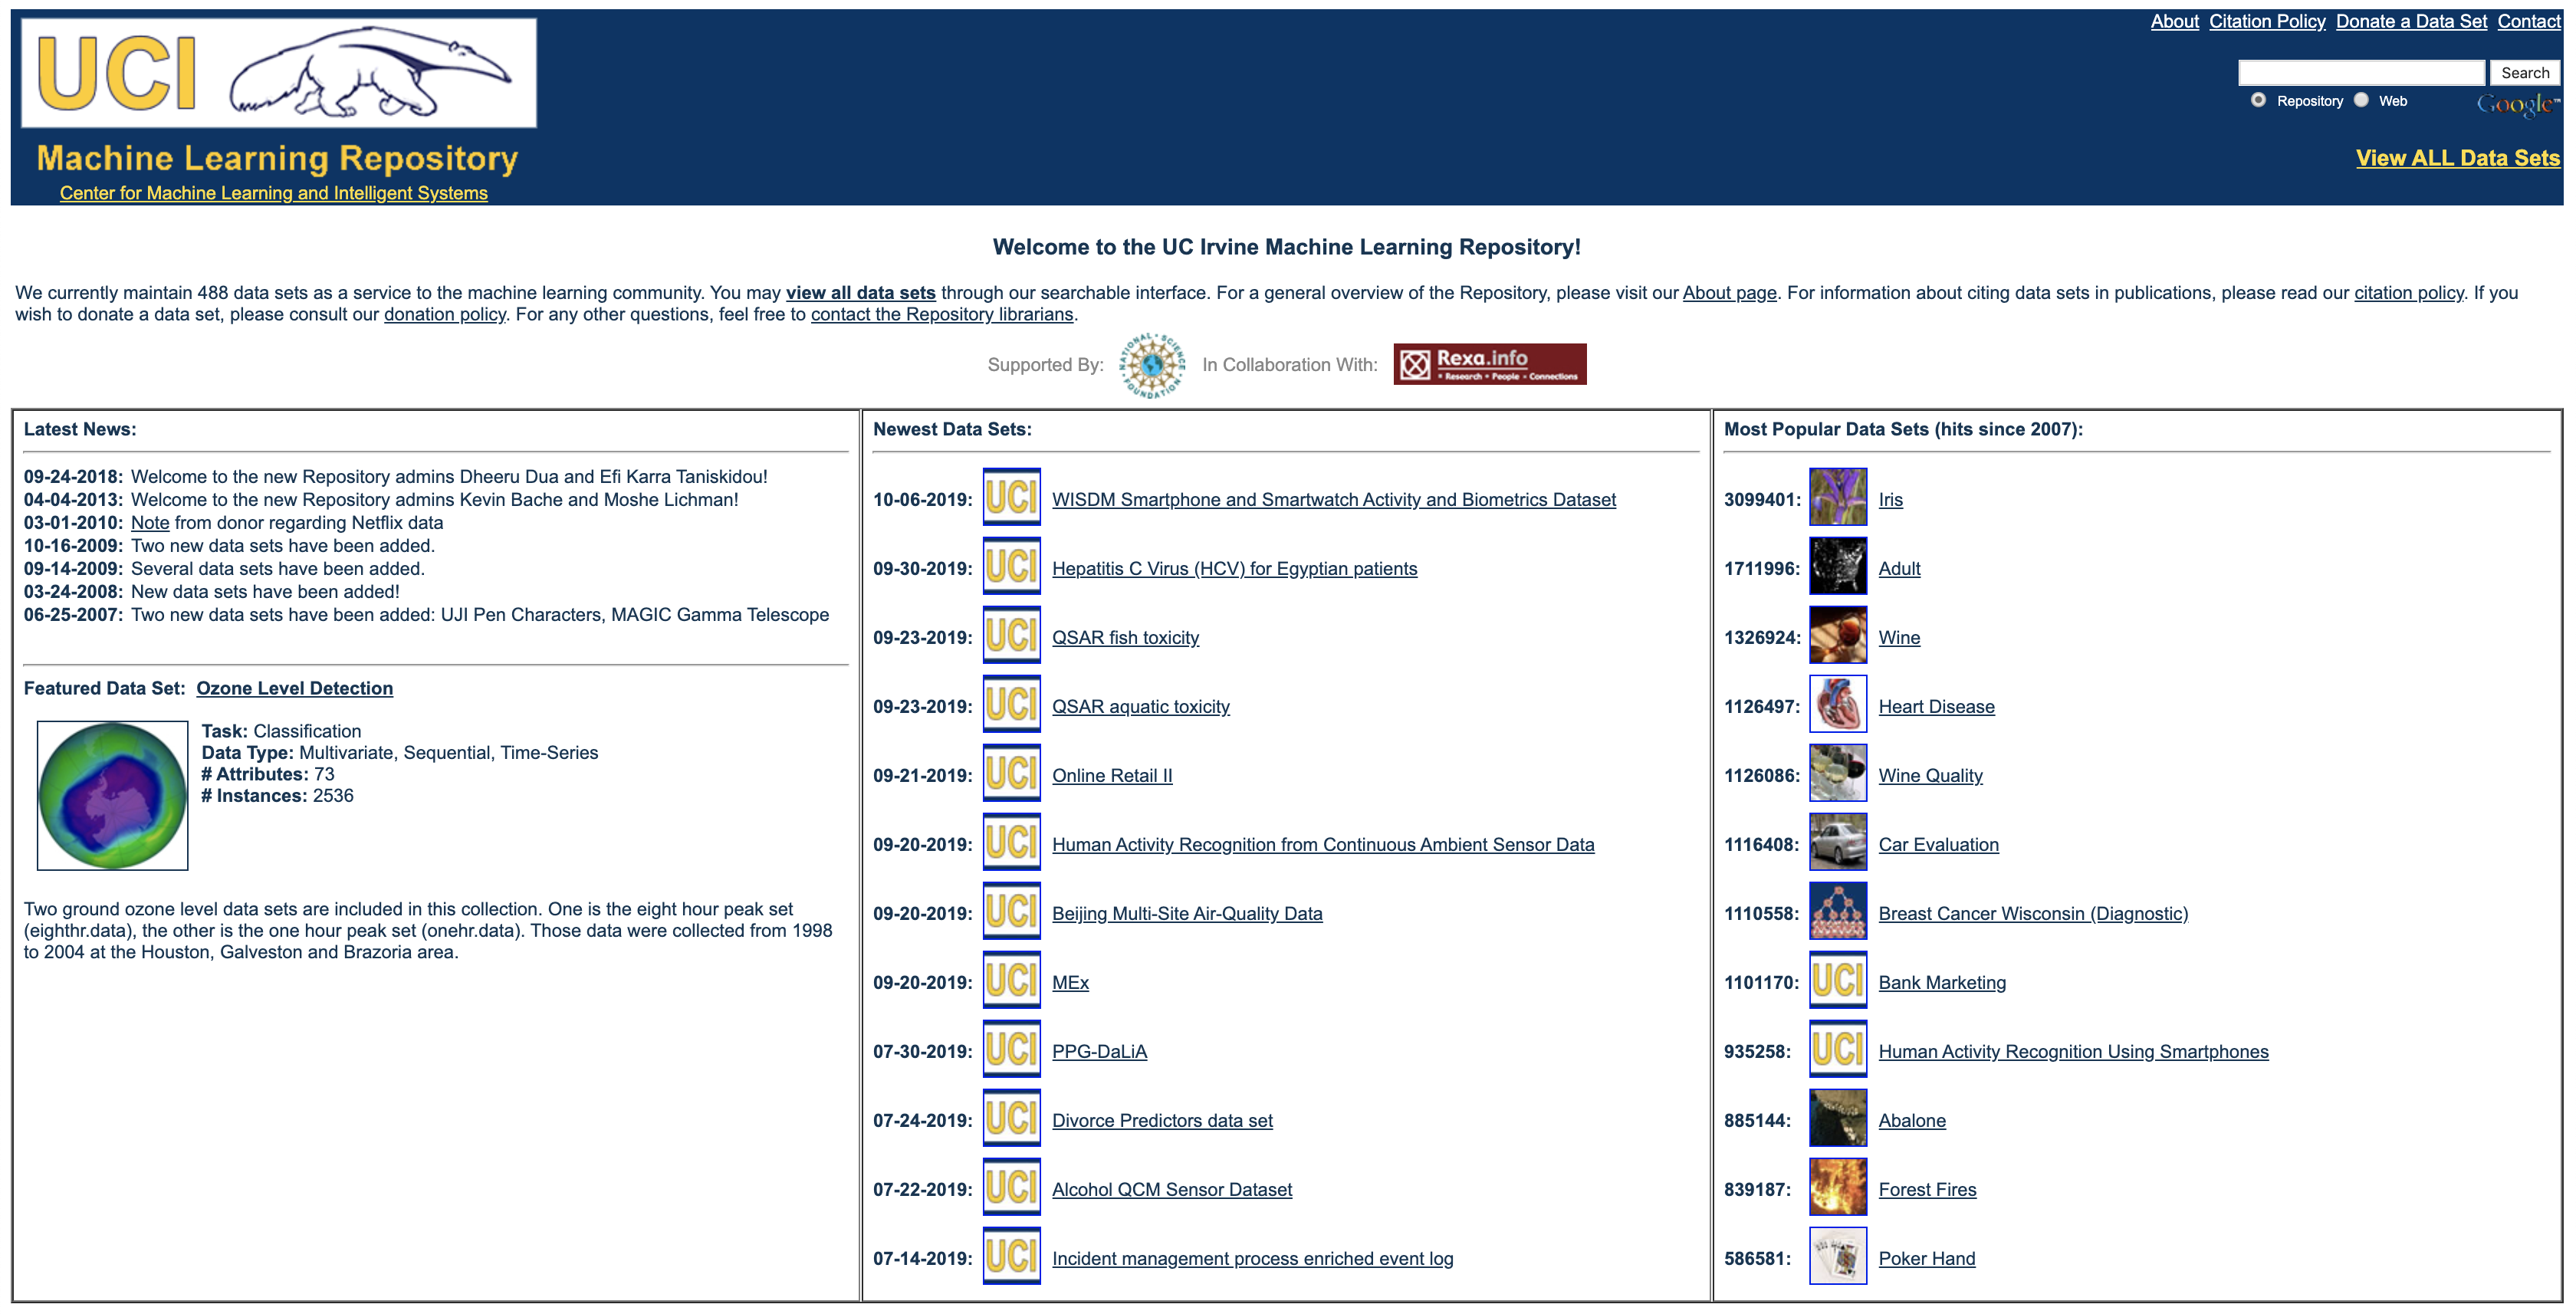
\includegraphics[width=\textwidth]{uci_image.png}
		
		\vspace{1em}
		\alert{\textbf{This place is a great resource for projects!}}
	\end{center}
\end{frame}

\begin{frame}
		\frametitle{predicting mpg}
		Datasets from UCI (and many other places) comes as tab, space, or comma delimited files. 
			\begin{center}
			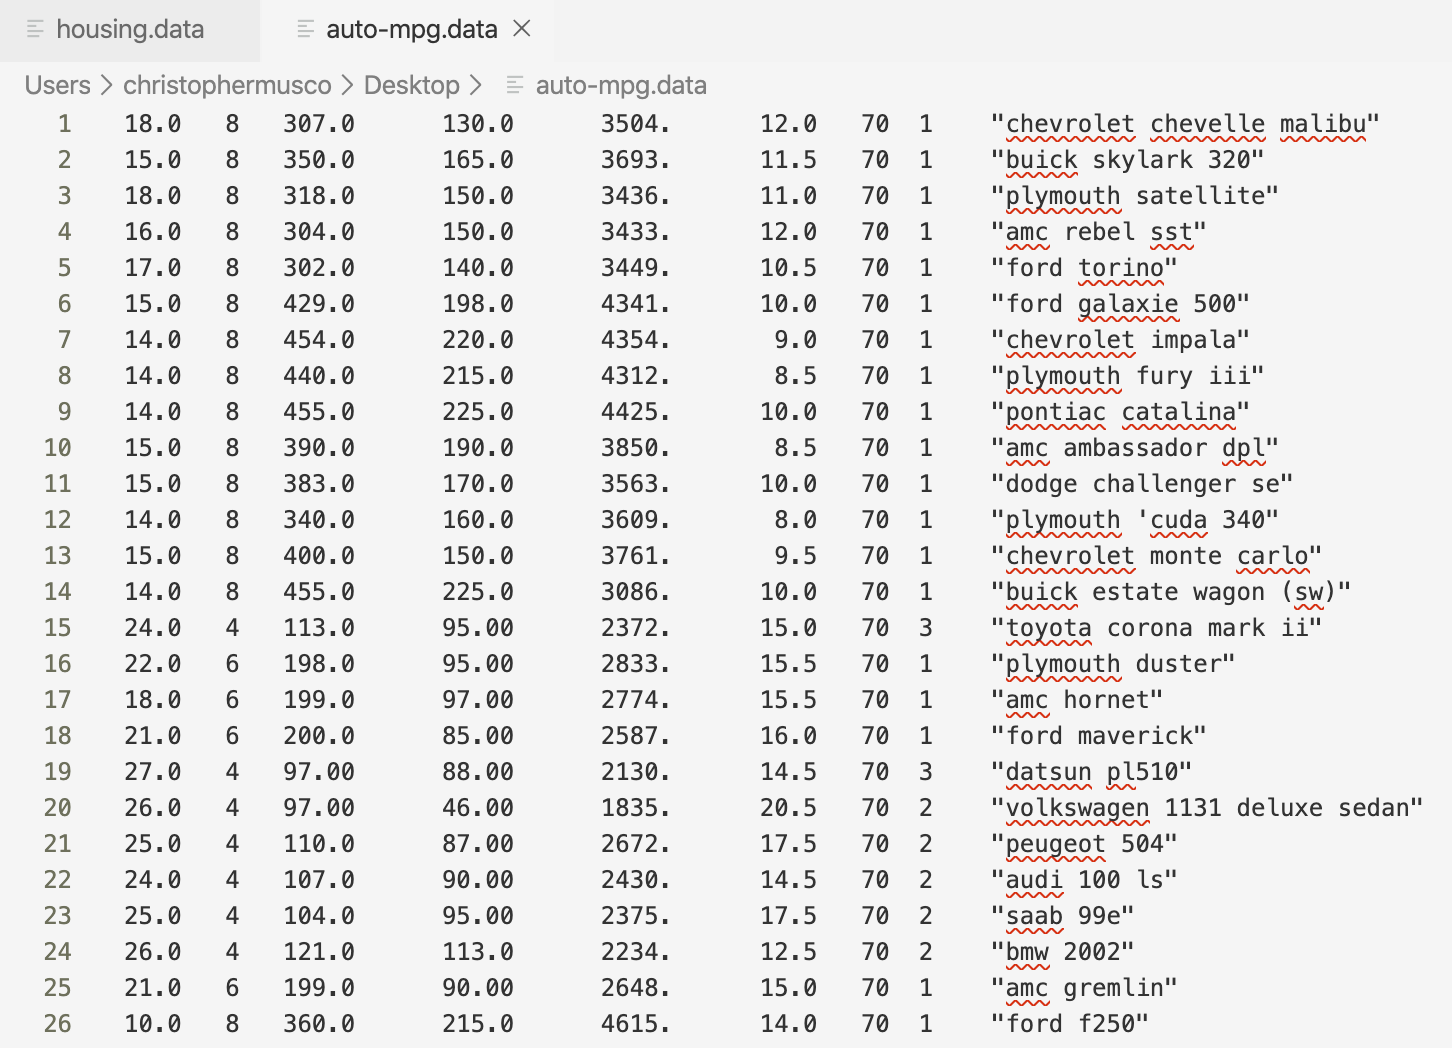
\includegraphics[width=.7\textwidth]{auto_data.png}
		\end{center}
\end{frame}

\begin{frame}
	\frametitle{predicting mpg}
	Check dataset description to know what each column means. 
	\begin{center}
		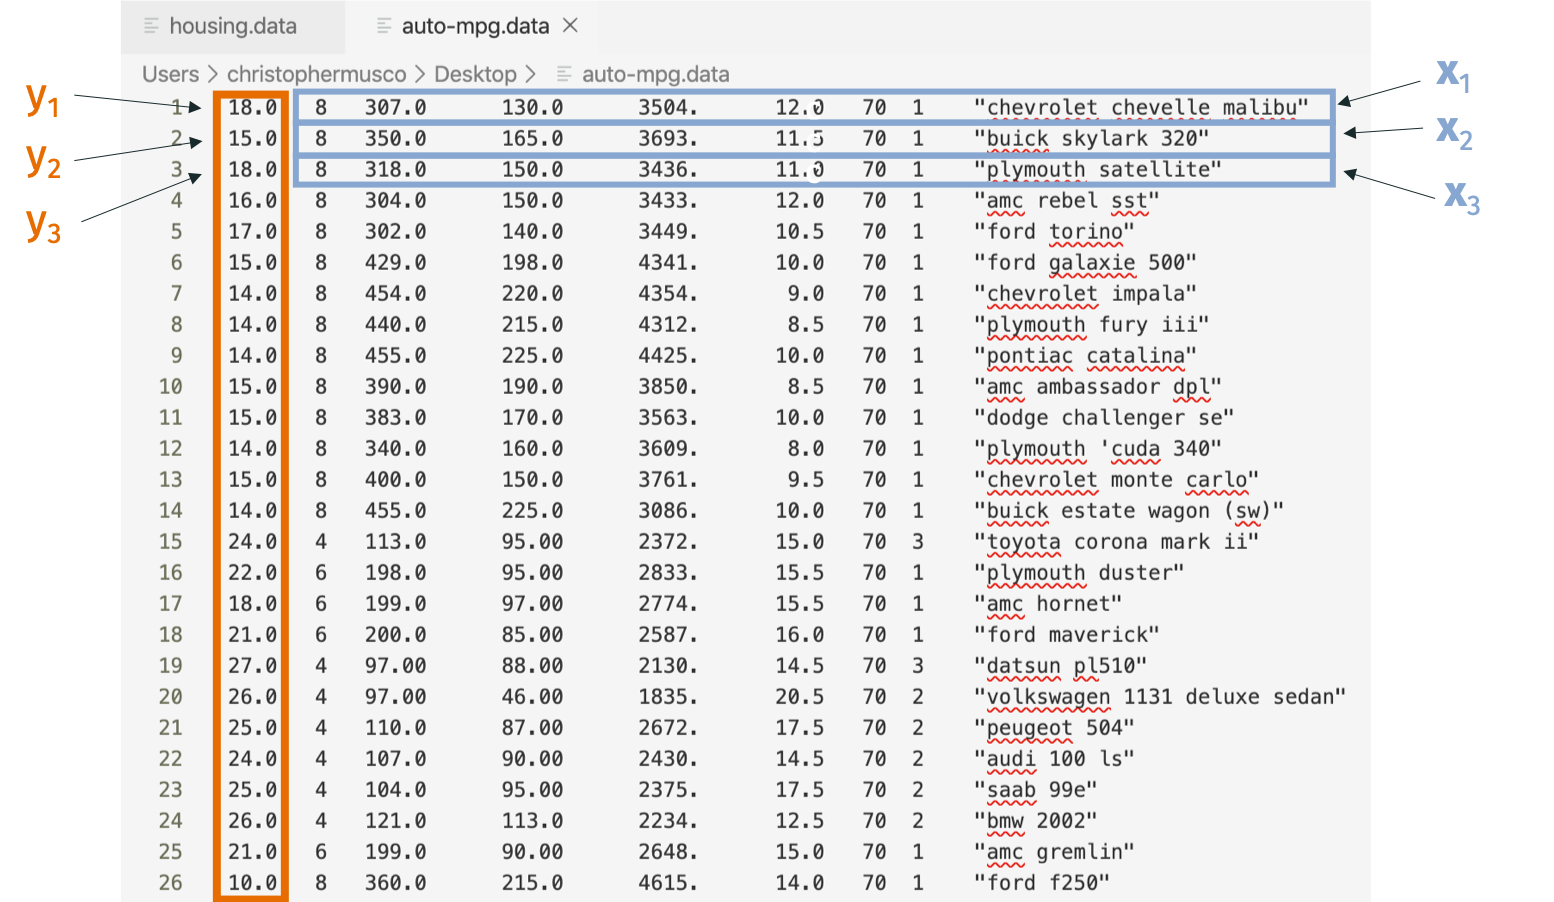
\includegraphics[width=.8\textwidth]{auto_data_marked.png}
		
		'mpg', 'cylinders','displacement', 'horsepower', 'weight', 'acceleration', 'model year', 'origin', 'car name'
	\end{center}
\end{frame}

\begin{frame}
	\frametitle{libraries for initial data reading}
	\begin{itemize}
		\item Use \texttt{pandas} for reading data from delimited files. Stores data in a type of table called a ``data frame'' but this is just a wrapper around a \texttt{numpy} array.
		\item Use \texttt{matplotlib} for initial exploration. 
	\end{itemize}
	\begin{center}
		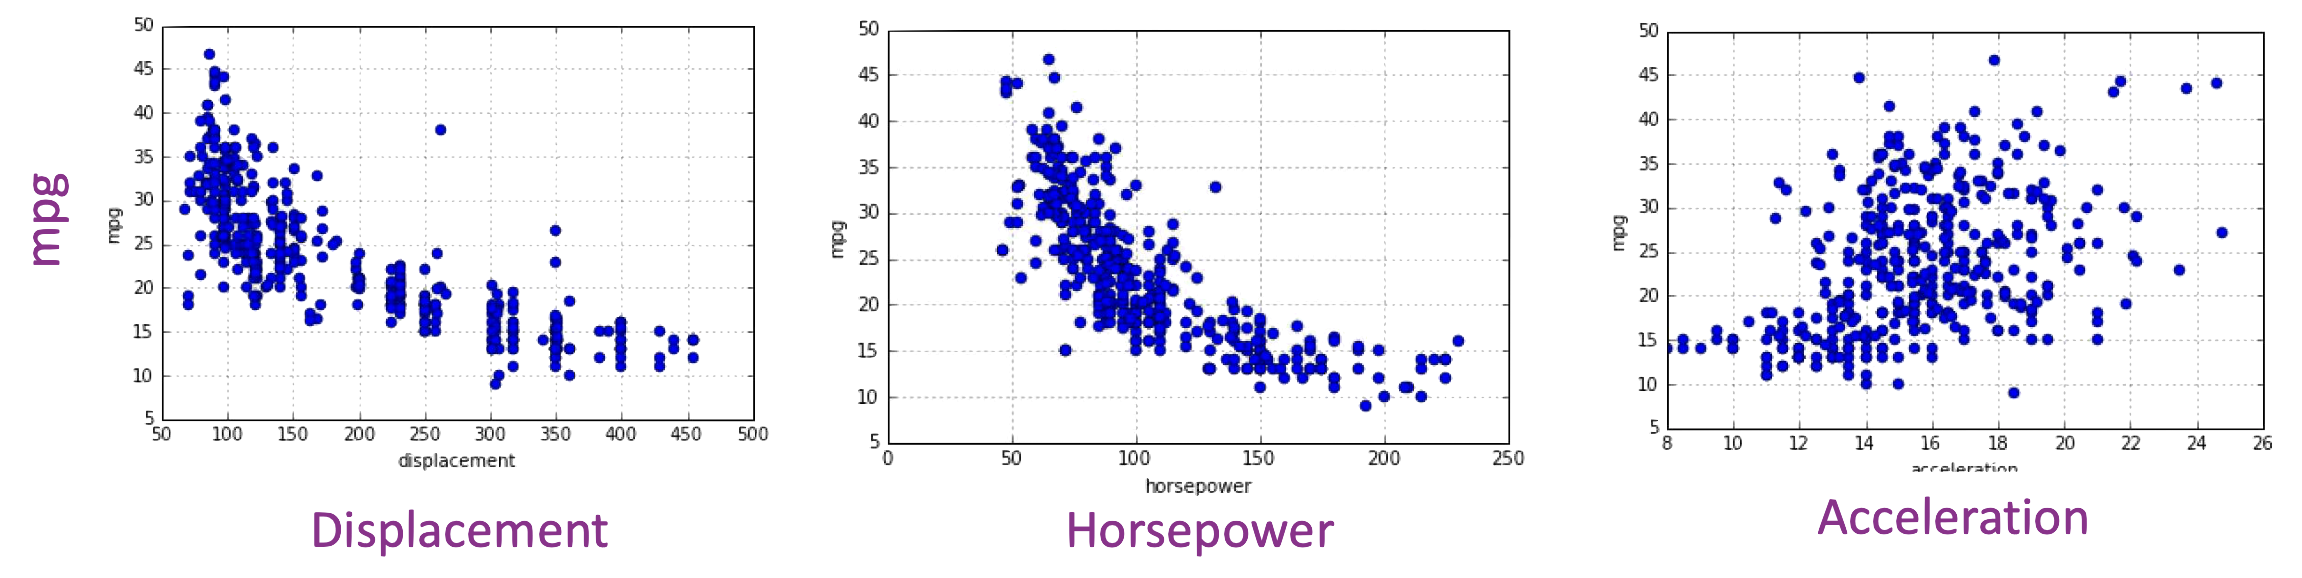
\includegraphics[width=\textwidth]{mpg_plots.png}
	\end{center}
\end{frame}

\begin{frame}
	\frametitle{simple linear regression}
	\textbf{Linear regression from a Machine Learning (not a Statistics) perspective.}
	Our first supervised machine learning model. 
	\begin{center}
		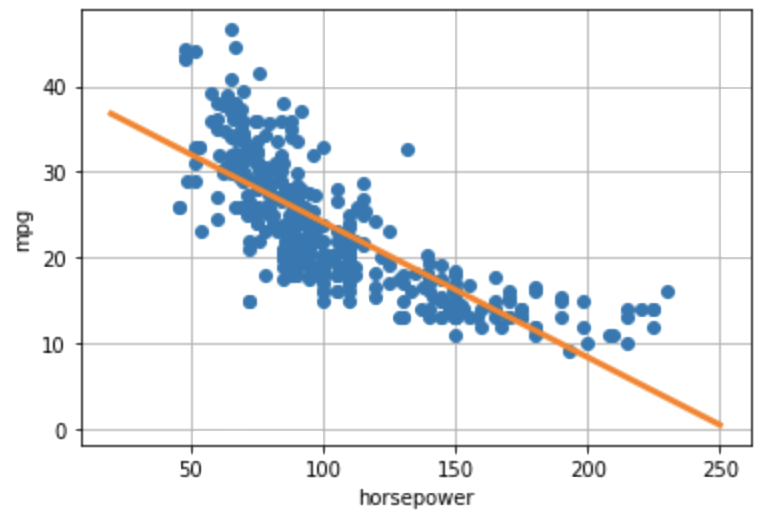
\includegraphics[width=.5\textwidth]{horsepower_fit.png}
		
		\vspace{-.5em}
		Only focus on \emph{one predictive variable} at a time (e.g. horsepower). 
		This is why it's called \emph{simple} linear regression.
	\end{center}
\end{frame}

\begin{frame}
	\frametitle{simple linear regression}
	\textbf{Dataset:} 
	\vspace{-.5em}
	\begin{itemize}
		\item $x_1, \ldots, x_n \in \R$ (horsepowers of $n$ cars -- this is the predictor/independent variable)
		\item $y_1, \ldots, y_n \in \R$ (MPG -- this is the response/dependent variable)
	\end{itemize}
	\begin{center}
		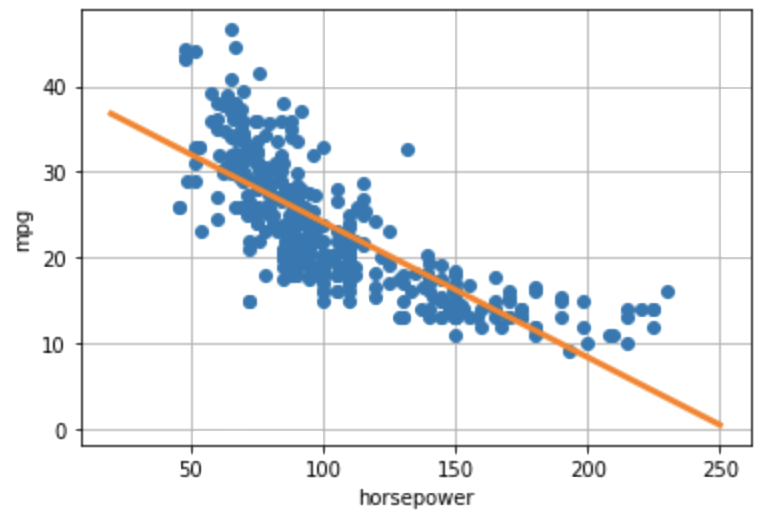
\includegraphics[width=.5\textwidth]{horsepower_fit.png}
	\end{center}
\end{frame}

\begin{frame}
		\frametitle{supervised learning definitions}
		\small
		\begin{itemize}
			\item \textbf{\alert{Model} $f_{\bs{\theta}}(x)$:} Class of equations or programs which map input $x$ to predicted output. We want $f_{\bs{\theta}}(x_i) \approx y_i$ for training inputs. 
			\item \textbf{\alert{Model Parameters} $\bs{\theta}$:} Vector of numbers. These are numerical nobs which parameterize our class of models.
			\item \textbf{\alert{Loss Function} $L(\bs{\theta})$:} Measure of how well a model fits our data. Typically some function of $f_{\bs{\theta}}(x_1) - y_1, \ldots, f_{\bs{\theta}}(x_n) - y_n$
		\end{itemize}
		\begin{center}
			\textbf{Goal:} Choose parameters $\bs{\theta}^*$ which minimize the Loss Function:
			\begin{align*}
			 	\bs{\theta}^* = \argmin_{\bs{\theta}} L(\bs{\theta})
			\end{align*}
		\end{center}
\end{frame}

\begin{frame}
	\frametitle{linear regression}
	\begin{columns}
		\begin{column}{.5\textwidth}
			\begin{center}
				\textbf{General Supervised Learning}
			\end{center}
			
			\begin{itemize}
				\item Model: $f_{\bs{\theta}}(x)$
				\vspace{4em}
				\item Model Parameters: $\bs{\theta}$
				\vspace{4em}
				\item Loss Function: $L(\bs{\theta})$
				\vspace{4em}
			\end{itemize}
		\end{column}
		\begin{column}{.5\textwidth}
			\begin{center}
				\textbf{Linear Regression}
			\end{center}
			
			\begin{itemize}
				\item Model: 
				\vspace{4em}
				\item Model Parameters: 
				\vspace{4em}
				\item Loss Function:
				\vspace{4em}
			\end{itemize}
		\end{column}
	\end{columns}
\end{frame}

\begin{frame}
	\frametitle{how to measure goodness of fit}
	What is a natural \textbf{loss function} for linear regression?
	\begin{center}
	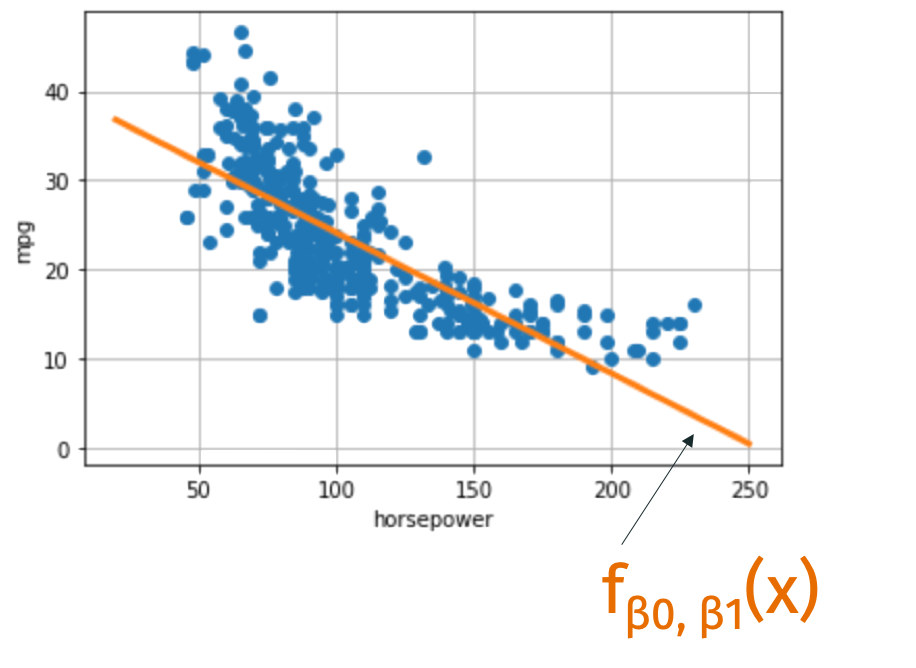
\includegraphics[width=.5\textwidth]{visualizing_fit.png}
	\end{center}
\end{frame}

\begin{frame}
	\frametitle{how to measure goodness of fit}
	\small
	Typical choices are a function of $y_1 - f_{\beta_0,\beta_1}(x_1), \ldots, y_n - f_{\beta_0,\beta_1}(x_n) $
	\begin{center}
		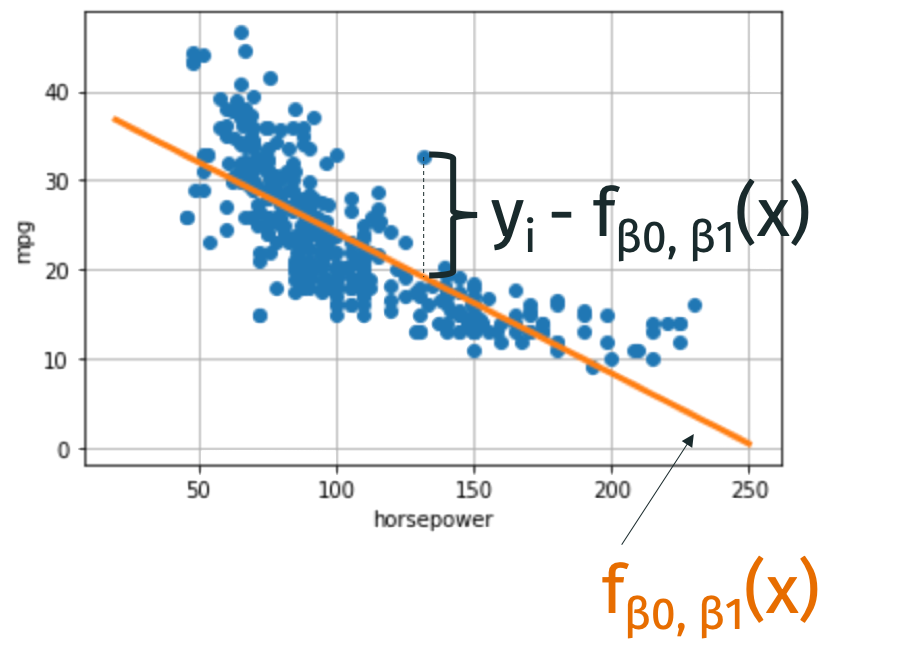
\includegraphics[width=.5\textwidth]{visualizing_loss.png}
	\end{center}
	\begin{itemize}
		\item $\ell_2$/\textbf{Squared Loss:} $L(\beta_0,\beta_1) = \sum_{i=1}^n \left[y_i - f_{\beta_0,\beta_1}(x_i)\right]^2$.
		\vspace{.5em}
		\item $\ell_1$/\textbf{Lease absolute deviations:} $L(\beta_0,\beta_1) = \sum_{i=1}^n \left|y_i - f_{\beta_0,\beta_1}(x_i)\right|$.
		\vspace{.5em}
		\item $\ell_\infty$ \textbf{Loss } $L(\beta_0,\beta_1) = \max_{i\in 1,\ldots, n} \left|y_i - f_{\beta_0,\beta_1}(x_i)\right|$.
	\end{itemize}
\end{frame}

\begin{frame}
	\frametitle{how to measure goodness of fit}
	\small
	We're going to start with the Squared Loss/Sum-of-Squares Loss. Also called ``Residual Sum-of-Squares (RSS)''
	\begin{center}
		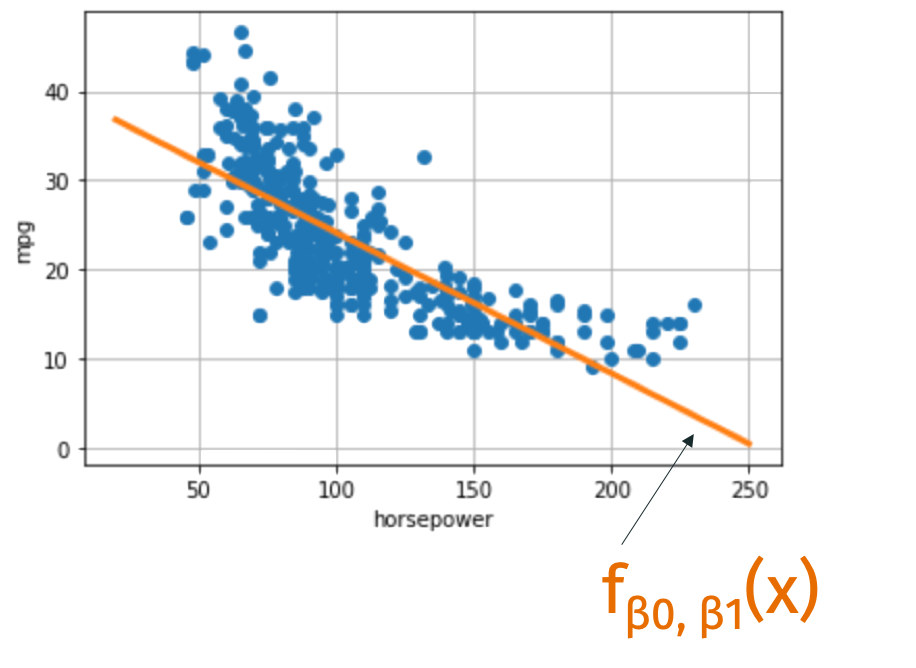
\includegraphics[width=.5\textwidth]{visualizing_fit.png}
	\end{center}
\vspace{-1em}
\begin{itemize}
	\item Relatively \emph{robust} to outliers.
	\item Simple to define, leads to simple algorithms for finding $\beta_0,\beta_1$
	\item Justifications from \emph{classical statistics} related to assumptions about Gaussian noise. Will discuss later in the course. 
\end{itemize}
\end{frame}

\begin{frame}
	\frametitle{linear regression}
	\begin{columns}
		\begin{column}{.5\textwidth}
			\begin{center}
			\textbf{General Supervised Learning}
			\end{center}
	
			\begin{itemize}
				\item Model: $f_{\bs{\theta}}(x)$ \hspace{20em}
				\vspace{2em}
				\item Model Parameters: $\bs{\theta}$
				\vspace{2em}
				\item Loss Function: $L(\bs{\theta})$ \hspace{20em}
				\vspace{2em}
			\end{itemize}
		\end{column}
		\begin{column}{.5\textwidth}
			\begin{center}
				\textbf{Linear Regression}
			\end{center}
		
			\begin{itemize}
			\item Model: $f_{\beta_0,\beta_1}(x) = \beta_0 + \beta_1\cdot x$
			\vspace{2em}
			\item Model Parameters: $\beta_0, \beta_1$
			\vspace{2em}
			\item Loss Function: $L(\beta_0,\beta_1) = \sum_{i=1}^n (y_i - f_{\beta_0,\beta_1}(x_i))^2$ 
			\vspace{2em}
			\end{itemize}
		\end{column}
	\end{columns}
\vspace{-2em}

\begin{center}
	\textbf{Goal:} Choose $\beta_0,\beta_1$ to minimize $L(\beta_0,\beta_1) = \sum_{i=1}^n (y_i - \beta_0 - \beta_1x_i)^2$.
	
	This is the entire job of any \textbf{\alert{Supervised Learning Algorithm}}.
\end{center}
\end{frame}

\begin{frame}
		\frametitle{function minimization}
		\textbf{Univariate function:}
		\begin{center}
			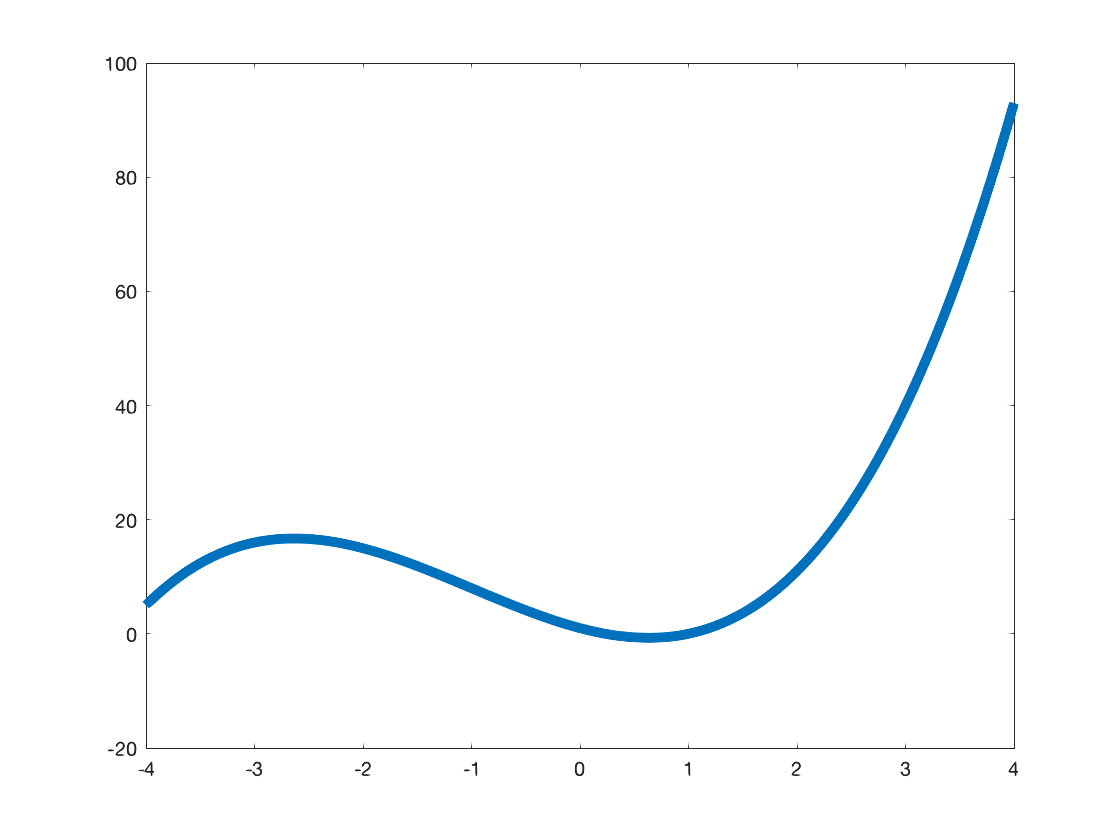
\includegraphics[width=.6\textwidth]{curve.png}
			
			$x^3 + 3\cdot x^2 - 5 \cdot x + 1$
		\end{center}
	\begin{itemize}
		\item Find all places where \emph{derivative} $f'(x) = 0$ and check which has the smallest value.
	\end{itemize}\end{frame}

\begin{frame}[t]
	\frametitle{function minimization}
	\textbf{Multivariate function:} $L(\beta_0, \beta_1)$
	\begin{itemize}
		\item Find  values of $\beta_0,\beta_1$ where \emph{all} partial derivatives equal $0$.
		\item $\frac{\partial L}{\partial \beta_0} = 0$ and $\frac{\partial L}{\partial \beta_1} = 0$.
	\end{itemize}

\end{frame}

\begin{frame}[t]
	\frametitle{minimizing squared loss for regression}
	\textbf{Multivariate function:} $L(\beta_0, \beta_1) = \sum_{i=1}^n (y_i - \beta_0 - \beta_1x_i)^2$
	\begin{itemize}
		\item Find  values of $\beta_0,\beta_1$ where \emph{all} partial derivatives equal $0$.
		\item $\frac{\partial L}{\partial \beta_0} = 0$ and $\frac{\partial L}{\partial \beta_1} = 0$.
	\end{itemize}
	
	\textbf{Some definitions:} 
	\begin{itemize}
		\item Let $\bar{y} = \frac{1}{n}\sum_{i=1}^n y_i$. \hspace{8.5em}$\bar{y}$ is the \emph{mean} of $y$. 
		\item Let $\bar{x} = \frac{1}{n}\sum_{i=1}^n x_i$. \hspace{8.5em}$\bar{y}$ is the \emph{mean} of $x$. 
		\item Let $\sigma_y^2 = \frac{1}{n}\sum_{i=1}^n (y_i - \bar{y})^2$. \hspace{5em}$\sigma_y^2$ is the \emph{variance} of $y$.
		\item Let $\sigma_x^2 = \frac{1}{n}\sum_{i=1}^n (x_i - \bar{x})^2$. \hspace{5em}$\sigma_x^2$ is the \emph{variance} of $x$.
		\item Let $\sigma_{xy} = \frac{1}{n}\sum_{i=1}^n (x_i - \bar{x})(y_i - \bar{y})$. \hspace{2em}$\sigma_{xy} $ is the \emph{covariance}.
	\end{itemize}
 \alert{\textbf{Claim:} $L(\beta_0, \beta_1)$ is minimized when:
 	\begin{itemize}
 	\item $\beta_1 = {\sigma_{xy}}/{\sigma_{x}^2}$
 	\item $\beta_0 = \bar{y}-\beta_1\bar{x}$
 	\end{itemize}}
\end{frame}

\begin{frame}[t]
	\frametitle{proof}
	
\end{frame}

\begin{frame}[t]
	\frametitle{proof}
	
\end{frame}

\begin{frame}[t]
	\frametitle{minimizing squared loss for regression}
	\textbf{Takeaways:}
	\begin{itemize}
		\item Minimizing functions is often easy with calculus. 
		\item Tools we will see again: \textbf{linearity of derivatives}, \textbf{chain rule}.
		\item Simple closed form formula for optimal parameters $\beta_0^*$ and $\beta_1^*$ for squared-loss!
	\end{itemize}
\begin{center}
	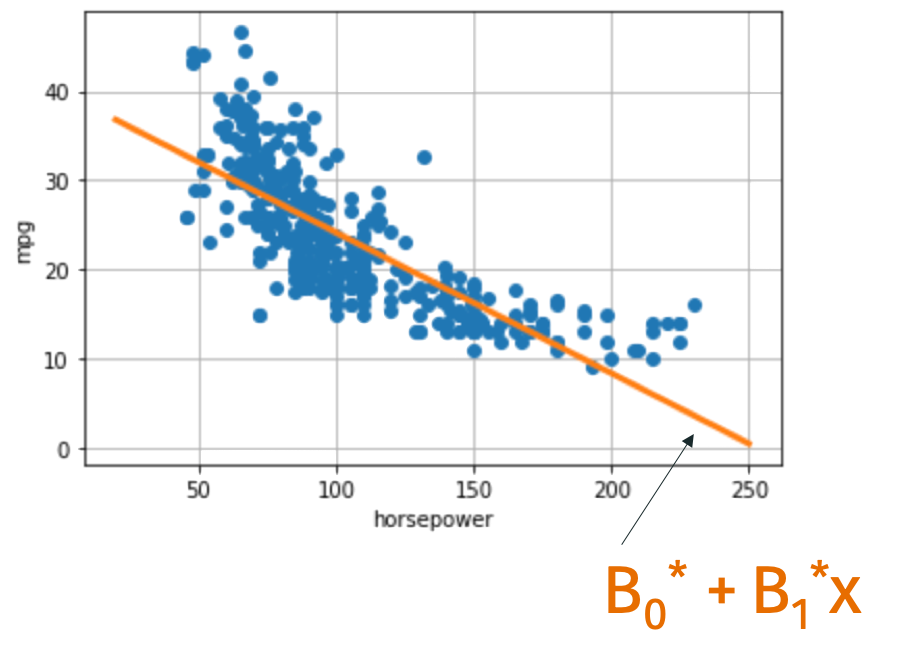
\includegraphics[width=.5\textwidth]{opt_final.png}
\end{center}
\end{frame}

\begin{frame}
	\frametitle{a few comments}
	Let $L(\beta_0,\beta_1) = \sum_{i=1}^n (y_i - \beta_0 - \beta_1x_i)^2$.
	\begin{align*}
	R^2 = 1 - \frac{L(\beta_0,\beta_1) }{n\sigma_y^2} 
	\end{align*}
	is exactly the $R^2$ value you may remember from statistics. 
	
	The smaller the loss, the closer $R^2$ is to 1, which means we have a better regression fit. 
\end{frame}

\begin{frame}[t]
	\frametitle{a few comments}
	\textbf{Many reasons you might get a poor regression fit:}
	\begin{center}
		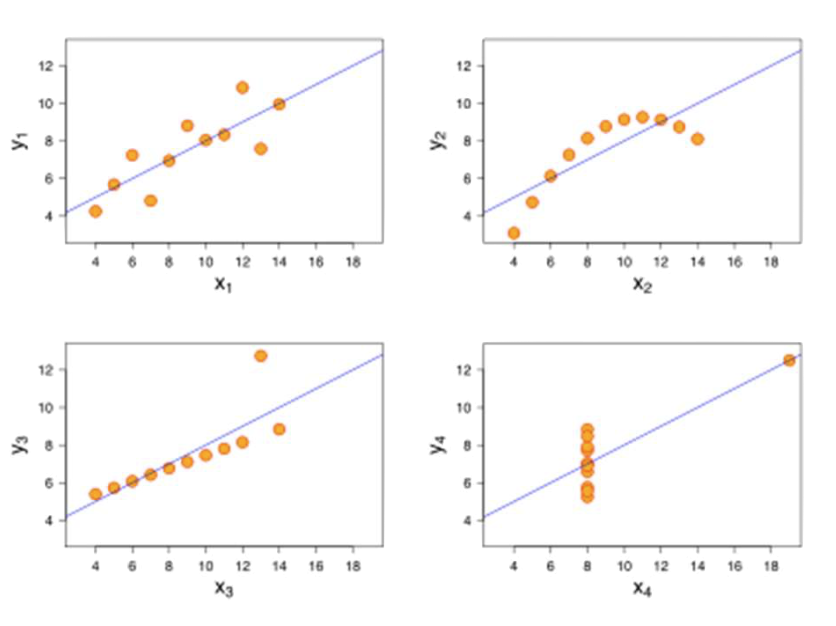
\includegraphics[width=.7\textwidth]{poor_fit.png}
	\end{center}
\end{frame}

\begin{frame}[t]
	\frametitle{a few comments}
	Some of these are fixable!
	\begin{itemize}
		\item Remove outliers, use more robust loss function.
		\item \alert{\textbf{Non-linear model transformation.}}
	\end{itemize}
	Fit the model $\frac{1}{\text{mpg}} \approx \beta_0 + \beta_1\cdot \text{horsepower}$.
	
	\begin{center}
		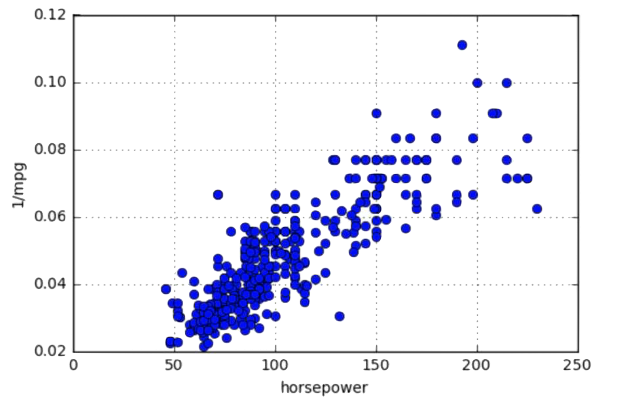
\includegraphics[width=.45\textwidth]{oneovermpg.png}	\includegraphics[width=.45\textwidth]{nonlinear_fit.png}
	
	\textbf{Much better fit, same exact learning algorithm!}
	\end{center}
	
\end{frame}

\end{document} 








